\documentclass{article}
\usepackage{tikz}
\usepackage{mathpazo}
\usepackage{xcolor}
\usepackage{verbatim}
\usepackage{calc}
\usepackage{ifthen}

% No indentation
\setlength{\parindent}{0cm}

\newcounter{row}
\newcounter{col}

\newcommand{\epilogue}[1][false]{
  \ifthenelse{ \equal{#1}{true} }{ \def\showanswer{true} } {\def\showanswer{false} }
  \begin{center}
    \ifthenelse{ \equal{\showanswer}{true} }{
      \large \it See you at Table Hamlet!
    }
    {
      Guess again
    }
\end{center}
  }

% Scaling factor for KenKen grid
\edef\puzzlescale{1.2}
\edef\numrows{4}
\edef\numrowargs{8}

\edef\theanswernum{4}

\def\showanswer{false}

\newcommand\setrow[\numrowargs]{
  \setcounter{col}{1}
  \foreach \n in {#1, #2, #3, #4} {
    \edef\x{\value{col} - 1}
    \edef\y{1 + \numrows - \value{row}}
    \node[anchor=north west,scale=0.65*\puzzlescale] at (\x, \y) {\n};
    \stepcounter{col}
  }
  \ifthenelse{\equal{\showanswer}{true} }{
  \setcounter{col}{1}
  \foreach \n in {#5, #6, #7, #8} {
    \edef\x{\value{col} - 1}
    \edef\y{1 + \numrows - \value{row}}
    \node[anchor=center, scale=\puzzlescale] at (\x+0.5, \y-0.5) {\n };
    \stepcounter{col}
  }
    }
             {
               % false - do nothing
             }
  \stepcounter{row}
}

\newcommand\boldh[3]{
  \edef\y{\numrows-#1}
  \edef\x{#2}
  \edef\z{\x + #3}
  \draw[very thick] (\x, \y) -- (\z, \y);
}

\newcommand\boldv[3]{
  \edef\y{\numrows-#1}
  \edef\x{#2}
  \edef\z{\y - #3}
  \draw[ultra thick] (\x, \y) -- (\x, \z);
}

\definecolor{shadegray}{gray}{0.75}

\newcommand\shadebox[2]{
  \edef\y{\numrows-#1}
  \edef\x{#2}
  \fill[shadegray] (\x, \y) rectangle (\x+1,\y-1);
}

\begin{document}

\begin{center}
  \large \textbf{Solution}
\end{center}

\medskip

\begin{minipage}[center]{0.58\textwidth}

  \bigskip
  
  \parbox{0.85\textwidth}{
    \it
  \noindent
    ``To be, or not to be?  That is the question.
    \phantom{``}To be, or not to be?  That is the question.
    \phantom{``}To be, or not to be?  That is the question.''
  }

  \bigskip

  \begin{enumerate}
    \setcounter{enumi}{\theanswernum-1}
    \item \textbf{Hamlet}, Act~II, Scene~iii
  \end{enumerate}


\end{minipage}
%
\begin{minipage}[center]{0.38\textwidth}
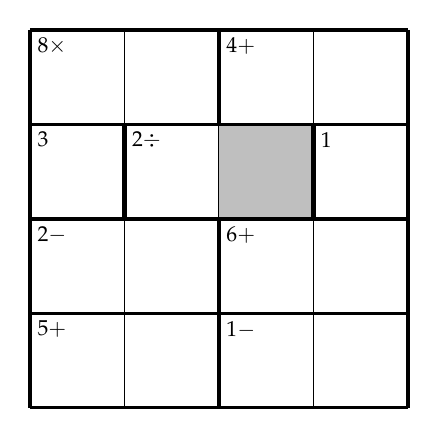
\begin{tikzpicture}[scale=\puzzlescale]

  \begin{scope}

    \shadebox{1}{2}
    
    \draw (0, 0) grid (4, 4);
    \boldh{0}{0}{4}
    \boldh{1}{0}{4}
    \boldh{2}{0}{4}
    \boldh{3}{0}{4}
    \boldh{4}{0}{4}
    \boldv{0}{0}{4}
    \boldv{1}{3}{1}
    \boldv{1}{1}{1}
    \boldv{0}{2}{1}
    \boldv{2}{2}{2}
    \boldv{0}{4}{4}

    \setcounter{row}{1}
    \setrow {$8\times$} {} {$4+$} {} {2} {4} {1} {3} 
    \setrow {$3$} {$2\div$} {} {$1$} {3} {2} {4} {1} 
    \setrow {$2-$} {} {$6+$} {} {1} {3} {2} {4} 
    \setrow {$5+$} {} {$1-$} {} {4} {1} {3} {2} 
    
    % \node[anchor=center] at (0.5*\numrows, -0.5) {Ken Ken};
  \end{scope}

\end{tikzpicture}
\end{minipage}

\bigskip

\epilogue[true]

\epilogue[false]

\end{document}
